\chapter{The Envoy Prototype}\label{cha:implementation}

Even the simplest file systems involve complex interactions between numerous hardware and software components, and distributed file systems compound that complexity. While all modern designs tend to draw heavily on prior work, the particular combination of classic components and new innovations that make up a new system like Envoy can only be validated with empirical results.

I have implemented a prototype of Envoy to make testing possible and to permit a level of refinement in the design that is only possible with practical experience. This chapter first details the goals and parameters of the prototype, then discusses aspects of the implementation that shed further light on the design, expose its limitations, or show how implementation choices have shaped the prototype.

\section{Scope and design coverage}

\subsection{Goals of the prototype}

The goals of the prototype are more modest than the goals of the Envoy design. The design addresses the storage needs of a complex system, and its suitability for the problem at hand is determined partly by how accurately the problem was described. Including appropriate features addresses some of the needs of service clusters, and only production experience can fully determine how successful some features are. Because this dissertation addresses only the storage aspect of the commodity computation problem, a complete evaluation must be deferred.

Other aspects of the design and its suitability for the intended task can be validated by testing an implementation of the file system, even in the absence of a complete service cluster environment. The prototype was implemented to allow empirical testing of the basic structure of Envoy, and to expose practical issues that could lead to refinement of the design. The design presented in the previous chapter reflects many lessons learned from the prototype implementation, and the next chapter presents measurements from using it.

The remainder of this chapter describes the artifact itself. The Envoy design calls for a client-server file system interface for connecting individual clients to the distributed system, but it does not require a specific one. The prototype is written to support a specific interface, and the rest of the prototype takes design cues from that interface. While the storage layer is under-specified in the general design, a prototype supporting the general interface and redundant layout required by Envoy was necessary for testing; its implementation is also described here.

\subsection{Implementation shortcuts}

The prototype is designed to validate the basic design and performance of the Envoy system. Features with little effect on performance, such as authentication schemes and recovery procedures, were omitted because their implementation would prove little. Other shortcuts in the implementation supported faster implementation at the expense of runtime performance. For a prototype this is an appropriate tradeoff, as validation of the overall design is more important than particular benchmark results. A few such shortcuts are described here.

\subsubsection{Synchronization}

The prototype uses a simplified concurrency model based on a few assumptions. Concurrent transactions are permitted and executed on individual processor threads, but only one is allowed to execute at any given time. A global lock is held by the running thread, and is released whenever a network or disk operation is invoked. This simplifies shared-memory management considerably, and is justified on the assumption that the processing time for transactions is dominated by I/O latency.

Deadlock is avoided by forcing transactions to release all held locks when an attempt to acquire a new one fails. The transaction then waits on a queue and is restarted when the contended object becomes available. This forces transactions to acquire all necessary locks before introducing any side-effects that cannot easily be rolled back, but in exchange it allows locks to be acquired in any order and simplifies lock management. Multiple-reader/single-writer locks are also available for controlling access to territories, so contention is mostly limited to concurrent operations on the same file.

\subsubsection{Caching}

The prototype runs under Linux or other Unix systems, and takes advantage of the buffer cache of its host rather than implementing its own cache. This is a deliberate choice rather than a shortcut, as it takes advantage of the ongoing refinement of the host operating system. This is in line with the goal of taking advantage of commodity hardware and software, where continuing improvements are expected over time. The cache can be managed by managing the VM that hosts the envoy services.

\subsubsection{Garbage collection}

The prototype is implemented in C and uses the Boehm-Demers-Weiser conservative garbage collector \cite{boehm}. Garbage collection is unusual in file system implementations, and may come at a performance cost, but it is useful for simplifying and speeding up the implementation of the prototype.

\section{The 9p protocol}

Clients access Envoy using a client-server file system protocol between the virtual machine of the client and that of the envoy service. While a custom protocol would offer the greatest flexibility, it would also make the implementation considerably more complicated and would have little value in demonstrating the viability of the design.

\subsection{Alternatives}

With Linux as the client operating system of choice, a few prominent options were available but ultimately rejected for the prototype.

\subsubsection{NFS version 3}

The NFS protocol is popular, simple, well-understood, and has a robust implementation. Most of the complexity is implemented in the client drivers, so servers can be quite simple. I also had experience with the protocol after implemented a stackable, copy-on-write file system (CoWNFS) for the XenoServers deployment project \cite{kotsovinos04b}.

For user mode servers generally and Envoy in particular, however, the stateless model of NFS complicates implementation. File handles assigned by the server and given to the client are expected to be immutable and always available (there are no explicit open and close operations), making it difficult to maintain pairings between active files and the envoy instances that own them. With transparent copy-on-write, these handles must either be cached indefinitely or inherently tied to the name of the file. Changing territory boundaries makes caching impractical, and allowing for higher-level directories to be renamed makes the latter difficult to make robust.

Security under NFSv3 is based on Unix user and group IDs, which proves to be an inflexible mechanism when diverse clients become involved. The ID space must be shared between clients that share file systems, or the server must provide a mapping service to reconcile the differences. While not an insurmountable problem, this can get unnecessarily complicated when a client mounts multiple file system images, many clients share some images, and parts of those images are forked from standard base images.

The caching model of NFS is entirely under the control of the client driver, which generally sends frequent \texttt{stat} requests to check if its cache is still current. Write operations are generally asynchronous, however, and the lack of control would have defeated the cache coherency guarantees that Envoy seeks to achieve. Caching at the client level would also prevent consolidation of duplicate caches as the physical machine level, another of the aims of the Envoy design.

\subsubsection{NFS version 4}

The most recent update to NFS addresses many of these concerns by introducing a stateful model and using leases to manage client caching. These client delegations could work well with Envoy, allowing private files to be cached by the client and shared files to be held back and cached by the envoy. More flexible file handles and explicit state management also a better match. NFSv4 would be an attractive candidate for a future implementation, but at the time the Envoy prototype implementation was started, it was still relatively immature and the supporting tools were complicated to use and poorly documented.

\subsubsection{AFS}

The Andrew File System is another popular client-server system with a mature implementation. It employs persistent caching at the client, which is a poor fit for the Envoy model, and it is not intended as a general-purpose protocol for implementing custom servers. Adapting it to a system with very different semantics and basic assumptions would negate the benefits of using an established protocol and implementation.

\subsubsection{FUSE}

The FUSE driver and tools support custom userspace file systems under Linux. The FUSE interface is modeled after the Linux VFS interface and exposes some of its complexity, but the main point against using FUSE for the Envoy prototype is that it is not a network-facing protocol. A userspace tool for the client would be required that would in turn connect to the envoy service across the virtual network device. Besides adding an unnecessary layer of indirection, this would complicate using Envoy as a root file system.

\subsubsection{Custom Envoy client driver}

Another possibility would be to implement a custom kernel driver for the Envoy client as well as the Envoy server. This would permit an exact between the expectations of the client and the semantics supported by the server. It would also permit optimizations precluded in standard drivers by the need to support a diverse range of servers.

Using a custom driver would have disadvantages, among them the need to divert time away from the server or to extend the total implementation time required. A custom driver would not be available in standard software distributions, either, requiring additional deployment effort for end users. Finally, a protocol would make evaluation more difficult by making it harder to isolate the costs of the Envoy deployment model from the costs of the protocol and client implementation. Being able to compare Envoy performance against other servers using the same client driver may penalize the overall performance, but it also allows a more detailed analysis of the results.

\subsubsection{9p}

The Envoy prototype is implemented using the 9p protocol from the Plan~9 operating system \cite{pike90,pike92}, which is specified in section 5 of the Plan~9 manual \cite{9man}. Plan~9 breaks from Unix semantics in many ways, so the Linux port of 9p has been extended to better support Unix semantics \cite{hensbergen}. The 9p protocol is intentionally simple. Individual connections are established for each user, and file ownership is tracked using user and group names, not numeric identifiers. The protocol includes no explicit support for client-side caching beyond the availability of file version tagging that could support NFS-style cache validation checks.

The 9p protocol is based around the thirteen messages listed in \tabref{tab:9p-messages}. Authentication is achieved through an arbitrary sequence of reads and writes to a special file handle established with the \texttt{auth} message, and after the server is satisfied the client can follow-up by attaching to a specific point in the file hierarchy. Access to the rest of the hierarchy is through \texttt{walk} messages that move new or existing file handles through the namespace, and normal operations that can then access files and directories through the associated file handles.

\begin{table}[tp]
\begin{center}
\begin{tabular}{lp{8cm}}
\textbf{Message name} & \textbf{Description} \\
\texttt{version} & Initial handshake; establish message size limits. \\
\texttt{auth} & Authenticate a user to mount a specific path name. \\
\texttt{flush} & Cancel a pending request. \\
\texttt{attach} & Mount a specific path for a specific user. \\
\texttt{walk} & Navigate directories and/or clone a file handle. \\
\texttt{open} & Open a file or directory. \\
\texttt{create} & Create a file or directory. \\
\texttt{read} & Read bytes from a file or entries from a directory. \\
\texttt{write} & Write bytes to a file. \\
\texttt{clunk} & Release a file handle and close the file. \\
\texttt{remove} & Delete a file or empty directory. \\
\texttt{stat} & Read attributes for a file. \\
\texttt{wstat} & Change a file's attributes.
\end{tabular}
\end{center}
\caption[Messages in the 9p protocol]{The messages in the 9p protocol. \texttt{version} and \texttt{auth} prepare a connection for an \texttt{attach} request, which establishes a single file handle. \texttt{walk} can clone or move existing file handles, giving access to the rest of the file tree. \texttt{flush} relates to an individual transaction, but all other messages operate relative to an active file handle.}
\label{tab:9p-messages}
\end{table}

\subsection{Mapping Envoy to 9p}

For basic file operations, an envoy acts like a 9p server to the client. The service connects over a virtual network device that connects the service VM to the VM hosting the envoy service. While the prototype uses a standard TCP connection for communicating, 9p supports any transport layer and could use an interface for virtual machine environments that swaps memory pages between VMs instead of copying data through the standard network protocol stack. While this has not yet been implemented for 9p servers, it is a potential optimization that could reduce the additional cost of retrieving data from the machine-level cache over retrieving it from an OS-level cache in an individual VM.

\subsubsection{File handles and state management}

When a file is owned remotely, the local envoy acts as a proxy server and forwards requests to the appropriate envoy. Like client connections, forwarded transactions are tracked relative to file handles owned by specific users.

File handles are tracked by small positive integers, which are unique in the context of a specific connection. When acting as proxies, envoys map client identifiers to \emph{remote identifiers}, which are unique for a given envoy instance. This allows envoys to combine all requests from their constituent survives when contacting a remote envoy, effectively making the envoy act like a single client. By making the identifiers unique for all outgoing requests from the envoy instead of for each local-remote envoy pair, no re-mapping is required when file handles migrate from one remote envoy to another during territory realignments.

\subsubsection{Security}

In 9p individual users mount the file system, and file identifiers are subsequently tied to a single user. The server authenticates a specific user and authorizes the creation of a specific file handle at mount time, and additional file handles are produced by cloning existing ones and walking the directory structure to find the desired files.

This system is simple and matches the distributed layout of Envoy well. Envoys trust each other, so authentication need not be repeated as clients cross territory boundaries. Identifying individual users instead of authenticating hosts and leaving user management to them also makes shared images easier to manage. A user or process on one client can connect to a shared image using its own credentials, without requiring administrative access even on its own virtual machine. Likewise, the administrative user can be restricted and treated like a normal user on a shared volume without requiring any specific trust in the client's operating system.

9p does not specify the protocol for authenticating users, but instead offers a mechanism for arbitrary exchanges to take place before a user succeeds in attaching an image. This allows flexibility in the server implementation, which may rely on the network address (which can be securely controlled in service clusters) in addition to security protocols that exchange credentials. Generic implementations are possible within the bounds of 9p, along with closer integration with the cluster administrative system.

\subsubsection{Caching}

9p does not explicitly manage caching, and the Linux client driver does not implement any client-side caching. This supports Envoy's model of consolidated node-level caching by forwarding all requests immediately to the envoy. No further configuration is necessary for clients.

Because all requests cross the virtual network device between a client VM and the envoy services, the efficiency of the protocol is important to the performance of the file system. 9p permits any transport layer to be introduced under its message protocol, so an implementation that avoids copying data through the network stack and instead swaps physical memory pages between two virtual machines is viable. The prototype does not implement this, but 9p would permit it as an optimization.

\section{Storage service}

The storage service implements the bottom half of the storage layer, which is essentially an independent, stateless object server. Each server that contributes storage space runs a single instance of the storage service to export an object-level interface.

The storage layer is under-specified. It is an essential part of a complete Envoy implementation, but object management systems are not the subject of this dissertation, which instead focuses on building a complete distributed file system above an object-storage layer. The artifact described here is a stub, offering enough support to complete and test the file system build above it, but not enough for a production setup.

The remainder of this section describes the protocol used by the storage servers, and discusses the implementation of the object store.

\subsection{Protocol}

The storage server protocol is implemented as an extension of the 9p protocol. It uses the same RPC mechanism and shares the same hand-shaking messages. Like 9p, it does not define an authentication protocol, but instead provides a framework for implementations to exchange credentials. In its intended setting, authentication could also be based solely on IP addresses, since the entire network is controlled and virtual machines can easily be prevented from spoofing their addresses.

\tabref{tab:storage-messages} lists the messages unique to the storage server. The \texttt{reserver} message lets an envoy request a range of previously unallocated object IDs for its later use. Since storage servers do not communicate with each other directly, envoys must agree to consult a single storage server in a particular replica group, i.e., among those servers storing a given range of object IDs, to prevent overlapping allocations.

\begin{table}[tp]
\begin{center}
\begin{tabular}{lp{8cm}}
\textbf{Message name} & \textbf{Description} \\
\texttt{reserve} & Claim a range of unallocated object IDs. \\
\texttt{create} & Create a new object. \\
\texttt{clone} & Copy an existing object, set copy-on-write flags for directories. \\
\texttt{read} & Read a byte range from an object. \\
\texttt{write} & Write a byte range to an object. \\
\texttt{stat} & Query an object's attributes. \\
\texttt{wstat} & Modify an object's attributes. \\
\texttt{delete} & Remove an object. \\
\end{tabular}
\end{center}
\caption[Additional message in the storage service protocol]{The messages in the storage service protocol. \texttt{reserve} returns a range of object IDs previously unallocated by the same storage server. \texttt{clone} copies an object, and if it is a directory it also sets the copy-on-write flag for all entries in the new copy. All operations except \texttt{reserve} are stateless, requiring an object ID as well as operation-specific parameters.}
\label{tab:storage-messages}
\end{table}

In a centrally-controlled cluster, assigning ranges of object IDs to storage servers and picking master replicas is a job best accomplished by a centralized, possibly replicated server. Likewise, coordinating bulk transfers of objects between servers to accommodate new nodes or compensate for failed machines is much easier to manage from a single location than to manage using a distributed protocol. Such tasks would be light work even when controlling many machines, because the events that require coordination occur infrequently. Unlike peer-to-peer systems, managed clusters can trust individual nodes and avoid distributing tasks that are better handled by centralized services.

The \emph{clone} operation, which copies an object from one given ID to another, is the only procedure that differentiates regular file objects from directory objects. When the attributes indicate that an object being cloned is a directory, the storage server will expect it to follow a particular format (described in \secref{sec:directory-format}) and will set the copy-on-write flags within each block as it makes the copy. It is not essential that this functionality be part of the storage service, indeed the clone operation itself could be implemented in terms of the other procedures. It is merely a performance optimization to avoid extra network round trips when possible. When a copy is required from one storage server to another (when the envoy is directed to create new objects on a different server than an existing object) a more conventional sequence of reads and writes must occur.

The other operations are straightforward, though it is worth noting that they differ from the related 9p operations in an important way: they require an object ID as a parameter instead of an active file handle. Envoys can make and break connections to storage servers as needed without losing any state. A pool of connections to frequently used storage servers is an obvious optimization, but is not strictly necessary.

\subsection{Implementation}

The storage service is implemented as part of the same executable as the envoy service. The two must be run as separate processes even on the same virtual machine, but since they share an executable image they can also run from the same shared memory blocks. Combining them is convenient because they share a lot of code.

The protocols for 9p clients, the storage service, and the envoy service are implemented as one single set of messages, only some of which are considered valid for each connection type. This allows shared code for network management, concurrent message dispatch, and numerous lower-level libraries. The code for storing objects on disk is also used by the envoy service for managing the persistent cache.

\subsubsection{Disk layout}

Each object is stored as a file in a normal Linux file system. Objects are stored in a hierarchy of directories, arranged to create a radix tree indexed by the object ID. In this scheme, a 64 bit object ID is broken into a series of smaller bit sequences, each of which (as a hexadecimal string) names a directory in the path to the object.

The least-significant bits of the object ID are used in constructing the file name. Each node name in the tree need only identify the few bits that distinguish the branch of which it is the root---the entire path taken together identifies the full ID of the object.

The number of bits partitioned into each directory level is significant. It is chosen to be the largest value $n$ such that a directory with $2^n$ entries named by hexadecimal strings encoding $n$ bits each will fit in a single disk block on the underlying file system. This structure turns the file system into a crude radix tree with block-sized nodes, and uses the OS buffer cache for the indexing structure in place of a custom cache.

The bit-splitting process starts with the least-significant bits and proceeds to the most-significant bits, ensuring that if any level of the index has a smaller fan-out factor than any other, it will be the root. This is for two reasons: squandering space in a single root block is preferable to wasting an equivalent factor of space in every leaf node, and less critically, changing the number of bits in the object ID for an existing object store can be done by manipulating a few entries at the root and leaving all other nodes untouched.

\subsubsection{Directories and metadata}

The number of bits from the object ID stored in the file name at the leaf node is also different from the higher-level directory nodes. While some of the object attribute fields are provided by the backing file system, others fields are stored as strings in the file name itself. File names are of fixed length, and encode both the bits that distinguish the object from its immediate neighbors and object attributes that are not easily stored as file attributes.

As with the interior nodes of the radix tree, the number of files in a leaf directory is chosen to keep the directory in a single disk block. When the system looks for an object, it reads the entire directory that will hold that object and caches the results. This gives it the precise file name for the object (along with the metadata stored in that name) and also primes the buffer cache with the directory block, so when the object file itself is accessed it will be located through the cached directory. In this way, extra attributes can be accessed from the file names without incurring extra disk seeks.

The attributes stored in the file names are the file mode and names of the user and group that own the file. The mode (including access permissions and the file type) cannot be freely read from and written to in its entirety in normal file systems, so encoding a device or a directory as a normal file requires storing the type somewhere else. While access permissions could be stored in the standard mode attribute, they would be honored by the underlying file system and would prevent unfettered access by the storage manager. User and group names in Envoy are stored symbolically, while most Linux file systems store them as numeric IDs, and again the file system's recognition of their semantic meaning would interfere with the storage manager. Storing any of these fields as a prefix to the actual file contents would violate block alignment assumptions that many clients make about file data, so an external mechanism was desirable.

While access to files in the object store is stateless, the access patterns of normal file system use are applicable to objects. Because of the persistent cache, entire files are often read in sequence, a common pattern for client operations as well. The storage service caches open handles to the most recently accessed files, both to avoid having to re-open them on each request and to avoid giving the backing file system a false hint that the file is no longer needed. Open file handles are kept on a strict LRU basis, as are the cached lists of file names in leaf-node directories mentioned above.

\subsubsection{Caching}

Envoy considers a write request finished when it is in the memory of the storage servers for all replicas. While this opens a window during which the data could be lost by a system crash, it is unlikely that multiple replicas would crash during the same window (assuming that nodes in the cluster are sufficiently isolated from each other). The storage server immediately passes all requests through to the underlying file system, and relies on the OS buffer cache to implement delayed writes. This is the simplest approach to implementation (use someone else's) but is also a sensible choice. Little would be gained by a custom solution, and this approach takes advantage of continuing improvements in the operating system. Indeed, taking advantage of continuing improvements in commodity hardware and software is one of the primary motivations for the this work.

\subsection{Limitations}

The storage server implementation is meant to be as simple as possible while still supporting realistic workloads. With the intention that a production design would take advantage of other work in object storage systems, the prototype neglects several important characteristics of a complete system.

Despite the absence of these essential features, the storage prototype does implement replicated storage with all the characteristics necessary to support the envoy layer. As that is sufficient for the stated purposes of this dissertation, the prototype is also considered sufficient.

\subsubsection{Security}

While the mechanism for authenticating envoys at connection time exists, no authentication is attempted in the prototype. From a performance standpoint, a challenge-response scheme or something similar would be a startup cost that is ignored in the prototype. It would be largely hidden by even a moderately-sized connection pool, but it would be present. In a controlled environment like a service cluster, a scheme based on IP addresses would be faster, simpler, and just as secure in practice. IP addresses could be assigned according to the role of the owner, so traffic from client VMs could be easily identified by all, and the VM hosting envoy and storage services could employ a firewall to prevent storage servers from ever seeing client requests.

\subsubsection{Replica groups}

The top half of the storage layer, i.e., the part that maps object IDs to storage servers, is essentially absent from the prototype. For any large deployment, a suitable disbursement of objects across storage servers is essential. Different degrees of failure protection may be desirable as well, with increased replication being available to clients at a premium cost.

\subsubsection{Redistribution}

When nodes are added or removed from the cluster, objects must be moved and copied to maintain a suitable replication factor. While I have stated that this could be controlled by a centralized service, no mechanism currently exists for copying directly between storage servers (other than systems such as \texttt{rsync} that bypass the storage service and go directly to its object store). These capabilities are critical to a system that will change over time, which is a basic characteristic of any realistic cluster deployment.

\subsubsection{Failure recovery}

Recovery of a crashed envoy node is addressed in \secref{sec:envoy-recovery}, but recovery of a failed storage node is an equally important problem. While redundancy allows the envoy layer to continue serving files, changes made during the downtime must be propagated to the restored node to ensure consistency, and nodes that do not recover must be replaced or their stored objects redistributed.

\section{Envoy service}

The envoy service runs on each node to form a single, distributed service across the cluster. It exports a view of the global namespace by acting as a 9p server to VM clients running on the same physical machine. Each instance assumes responsibility for specific territories, or subsets of the namespace. The name \emph{envoy} comes into play in two respects: it negotiates contact between local clients and the larger system, and acts as representative for its local territories to other nodes in the cluster and their constituent clients.

This section starts by describing the protocol used for inter-envoy communication, and then proceeds to discuss some internals in the envoy implementation. This includes details about basic file operations and navigation between envoy instances, the copy-on-write mechanism behind the fork and snapshot operations, and the coordination of state during territory boundary realignment.

For operations that require the synchronous cooperation of multiple envoy instances, dependency cycles and deadlock become a concern. To minimize these issues, Envoy is designed with a top-down locking protocol where synchronous operations only directly involve immediate neighbors in the tree of territories, and owners of parent territories always initiate and coordinate transactions with those lower in the tree. While operations with wide-ranging impact may require communicating with every node in the cluster, they never require a cycle in the connectivity graph and are not prone to distributed deadlock.

\subsection{Protocol}

As with the storage service, the envoy services protocol is implemented as a series of extensions to the 9p protocol. The integration is closer at the envoy level, however, as forwarded transactions from remote clients use the standard 9p messages when appropriate, depending on the extensions listed in \tabref{tab:envoy-messages} mainly to implement territory management and handle operations that straddle territory boundaries.

\begin{table}[tp]
\begin{center}
\begin{tabular}{lp{8cm}}
\textbf{Message name} & \textbf{Description} \\
\texttt{snapshot} & Take a snapshot of a territory. \\
\texttt{nominate} & Request that the parent transfer control of a territory. \\
\texttt{grant} & Give the target control of a territory. \\
\texttt{revoke} & Reclaim control of a territory. \\
\texttt{migrate} & Inform an envoy of file handles that have moved. \\
\texttt{walkremote} & Change directories across a territory boundary. \\
\texttt{statremote} & Query file attributes across a territory boundary. \\
\texttt{closefid} & Release an old file handle after it has walked to a new host. \\
\texttt{renametree} & Inform descendents of a directory that has been renamed.
\end{tabular}
\end{center}
\caption[Additional messages in the envoy service protocol]{The messages in the envoy service protocol. The first five support the major state management operations, while the remainder handle cases where an operation affects multiple territories.}
\label{tab:envoy-messages}
\end{table}

Envoys establish connections with each other only when they need to, specifically when they have neighboring territories or when transactions from one envoy's clients involve a territory owned by another envoy. Neighboring territories always form a tree structure, with one territory in every pairing (and by extension its envoy) being considered the parent of the other.

New connections between envoys must be authenticated in a way similar to connections between envoys and storage servers. The handshake messages from 9p are used, with the protocol string in the \texttt{version} message identifying the connection as one between envoys so that the appropriate range of messages will be understood. Authentication can proceed through an exchange of credentials, or the controlled environment of the service cluster can be exploited and network addresses can be used to identify authorized service hosts.

9p messages from \tabref{tab:9p-messages} are all considered valid coming from other envoys, with the exception of the \texttt{walk} and \texttt{attach} messages, which are replaced by an augmented version called \texttt{remotewalk} that accommodates territory boundary changes. Transactions still proceed in relation to normal file handles, with the further restriction that an envoy will never forward requests as a proxy for another envoy, only for clients.

\subsection{Data structures}

Unlike the stateless storage servers, envoy instances must track two main classes of state related to the two main roles an envoy assumes, namely those of 9p file server and territory owner.

\subsubsection{Territories and claims}

\begin{figure}[tp]
\centering
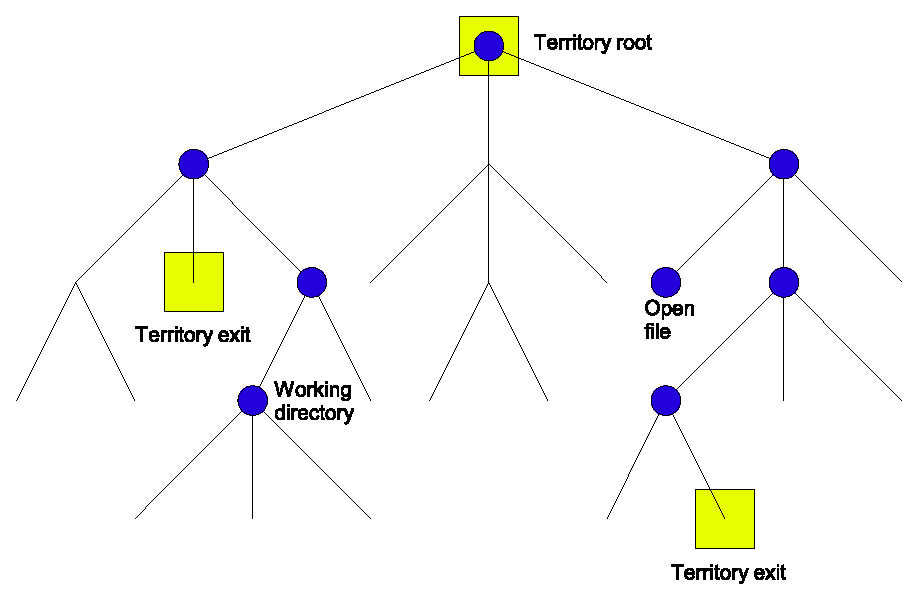
\includegraphics[width=\figwidth]{figures/territory-claims}
\caption[A territory managed by a single envoy]{Territories are trees, and their boundaries (yellow squares) are defined by the root pathname and the exits, which point to child territories owned by remote envoys. Claims (blue circles) represent individual storage objects, and within a territory they form a tree covering a subset of the territory, with leaves at each territory exit and active file or directory.}
\label{fig:territory-claims}
\end{figure}

An envoy may own zero or more territories, each of which is a branch of the global file tree, possibly with exits to child territories owned by other envoys as depicted in \figref{fig:territory-claims}. When the territory is given to the envoy through a \texttt{grant} message, it is also given the object ID that currently backs the root directory or file (a territory can be a single file) and a flag indicating if the object is writable. A territory may cover a snapshot image, in which case all objects are read-only. The root of the territory is never flagged as copy-on-write, so thaw operations (described in \secref{sec:freeze-thaw}) can always operate locally.

Overlaid on the file tree within a territory is another tree of \emph{claims}, or references to storage layer objects. Claims are maintained for all file handles, territory exits (actually the immediate parent directories of exits), and the path from any other claim back to the root of the territory. It is possible for multiple claims to exist for a single storage object, but only when the claims are all read-only or copy-on-write, and thus the associated objects are read-only. In this case, coordination for accessing the object is not necessary, and the file cache will recognize them as the same object to avoid duplication.

\subsubsection{File handles}

\begin{figure}[tp]
\centering
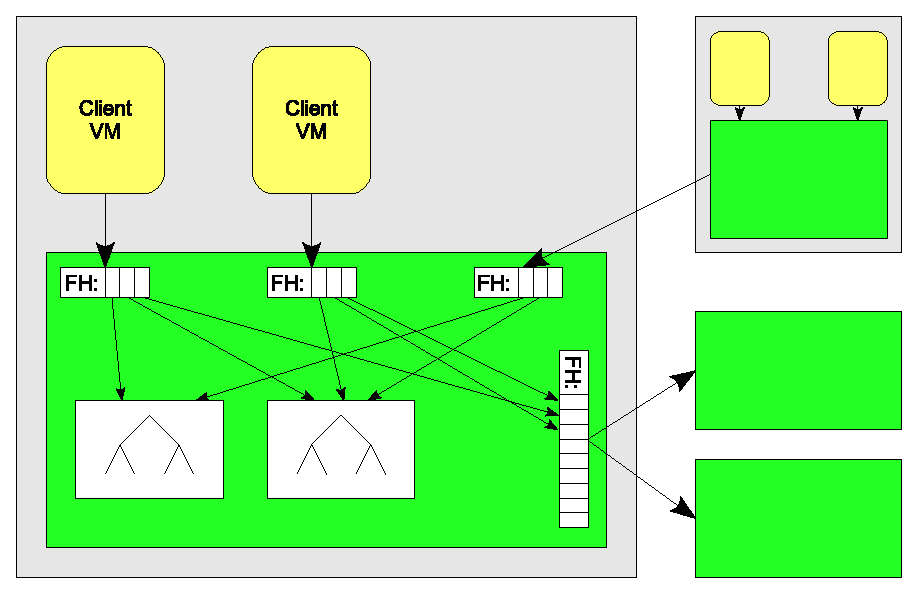
\includegraphics[width=\figwidth]{figures/file-handles}
\caption[Managing file handles in local and remote envoys]{File handles for incoming connections are grouped and distinguished by the source, be it a client VM or a remote envoy. Each handle is tied to a specific claim in a local territory. Client handles may also be forwarded to a remote envoy, in which case it is assigned an entry from the envoy's single remote file handle pool.}
\label{fig:file-handles}
\end{figure}

File handles in 9p are identified by small positive integers picked by the client, so the envoy interprets them in relation to the incoming connection. This gives each client a separate namespace, preventing confusion when resolving file handle IDs to file handles. All clients represented by a remote envoy are combined into a single ID space, so the envoy receiving the requests treats the entire envoy and all the clients is represents as a single client, as illustrated in \figref{fig:file-handles}. Since the user credentials are associated with individual file handles, this does not confuse security handling. Envoys-as-clients are not quite like regular clients, as their file handles are never re-forwarded; instead, when a file handle moves to a new territory the handle is sent back to the original envoy, which can forward it directly to the appropriate target.

When forwarding client requests for remote territories, the envoy re-maps the client ID to an envoy-specific remote ID. A single pool of remote IDs serves all outgoing connections, regardless of their targets, which simplifies territory migration as described in \secref{sec:migrating-state}. The envoy also maintains a local file handle stub for remote files, which is kept up-to-date by peeking at the requests and responses for remote operations. In this way, state for local clients is lost when an envoy fails, but state for remote envoys and their clients is preserved and can be used to recover from the failure.

\subsubsection{Persistent cache}

The persistent cache is the other major source of state in an envoy. On-disk objects are managed using the same code as the storage service uses for managing the object store, with the same disk structure and the same reliance on the underlying file system for in-memory caching.

The significant difference between the cache that an envoy maintains and the object store tended by a storage server is that the envoy must determine which objects are properly synchronized with the storage layer. Validating an unknown entry (one found in the persistent store but whose status is unknown) can be accomplished with a simple metadata comparison, so it is worthwhile keeping old objects even when the envoy has ceded the territory that referenced them, as it may eventually come back. Objects can be cleared when deleted, or based on a least-recently-used strategy. Once an object has been validated in the context of a territory that owns the object, it's validity need not be refreshed until the object has left local control.

\subsection{Freezing and thawing}\label{sec:freeze-thaw}

Synchronization at the object level is governed by an important invariant: an object in the system may be referred to by exactly one name in the hierarchical namespace, or it must be read-only. The storage layer makes no attempt to detect or enforce the read-only case, so it is left to the envoy layer to ensure that this invariant is preserved. To make this straightforward, objects can transition from being writable to read-only, but they can never go back. Note that this refers only to objects in the storage layer, not to the access control of file system objects.

The same invariant makes cache management simple: the envoy that owns a given territory can cache it without any invalidation concerns, and read-only objects can be safely cached at any number of envoy nodes without fear of interference. Objects in the cache become invalid only when a territory boundary changes. Objects that are part of ceded territory are not explicitly flushed from the cache; keeping them active helps in two cases: a read-only object may still be referenced by another name in a local territory, and the cache entry (in-memory or on-disk) may still be useful if a file backed by that object is later returned to local control. In the latter case the object must be verified to match the version in the storage layer, but this can be done with a lightweight metadata comparison.

The single mutable/multiple immutable dichotomy in the storage layer is tracked in the envoy layer through the copy-on-write flag in directory entries. The immutable property is not directly assigned to objects, but instead is imbued by the link from directory to file object. Furthermore, when the immutable object is itself a directory, the property is applied recursively to all of its children, overriding the individual copy-on-write flag in the link to each child. To be regarded as mutable, an object must be reachable by a path from the root of the global namespace to the directory entry linking to the object without traversing any copy-on-write flags that are set.

One immediate consequence of this is that taking a read-only snapshot of a directory and its descendents requires only setting the copy-on-write flag in the link to it, an operation known as \emph{freezing}. Once a directory or file is frozen, the storage layer objects that back the branch rooted at that point are considered immutable. To simplify bookkeeping, this operation is only performed from the root of client images when a snapshot operation is requested. The benefits gained from this restriction and an exception to it are discussed in \secref{sec:hard-links}.

The complementary operation is called \emph{thawing}. While the freeze operation works at the root of a subtree and affects it in its entirety, thawing aims to leave as small a footprint as possible; it is always performed with the goal of modifying a particular file. To thaw a file, the owning envoy starts walking up the line of its ancestors until it finds one that is already thawed. As the root of the namespace cannot be frozen (one can consider it as having a single, implicit link from the envoy service itself, but there is no mechanism provided to set the copy-on-write flag on this implicit link), this search is guaranteed to succeed. From there the envoy walks back to the target file, \emph{cloning} intermediate directories as it goes. In addition to making a copy of the directory as its name implies, cloning sets the copy-on-write flag of every directory entry in the copy, effectively transferring the copy-on-write property from the single link leading into the directory to all the links leading out of the directory. The implicit property that each child inherited becomes explicit after being passed down a generation. After thawing each directory for mutability, the parent is updated to reflect both the new object ID and the cleared flag. Eventually the intended target itself (be it file or directory) is cloned, its immediate parent link updated, and the file is fully thawed.

Thawing resembles the procedure for modifying a value in a tree in a functional language. In addition to changing the value itself, the path from that item to the root of the tree must be copied if the item is to be reachable from the root. In the thawing operation, it is only the root of the immutable subtree in which the item resides that must be copied. While the analogous procedure in a functional language copies everything exactly except for the path being changed, the thaw operation must clear the copy-on-write flag as it goes, and thus must push it down from parent link to sibling links at each level in order to preserve the immutable status of the unaffected branches.

The prototype clones an entire object, but it could be optimized to store deltas or otherwise compress changes, especially in directories and other metadata \cite{soules}.

\subsection{Read operations}

Most basic file and directory operations have a straightforward implementation. The need to cross territory boundaries makes some more complex, however, as they must coordinate with remote envoys to complete.

\subsubsection{Reading files and attributes}

The most straightforward operations are \texttt{read} and \texttt{stat}, which read the data and metadata of files, respectively. These requests can be filled using the data paths described in \secref{sec:data-paths-read}. The only complication involved is handling the \texttt{atime} attributed, which tracks the last time the data from a file was accessed by a \texttt{read} or \texttt{write} operation. Read operations always proceed through a single envoy, so this attribute can be tracked accurately: the envoy can send a message with the time stamp (to ensure that it is consistently applied to all replicas, even if all clocks are not in sync or network latencies between the different storage servers vary) to all replicas in the storage layer which can then update the attribute.

The intended meaning of the \texttt{atime} attribute becomes obscured when applied to frozen files, however. Since attributes are part of the object, akin to \texttt{inodes} in traditional Unix file systems, changing the attribute will affect all files that are backed by that same object. Those instances may be in read-only snapshots of the same file system image, or in common files available in an unrelated file system image. In the former case, the read-only property of the snapshot is broken, and in the latter case the isolation of the two images is compromised. Updating the \texttt{atime} attribute would give an unrelated client using the same prepackaged file system image the ability to loosely track file accesses, which could represent a security risk.

Accurately tracking the \texttt{atime} attribute is problematic with frozen files, and if it is only updated on some files (which may change over time as successive snapshots are taken), it is too unreliable to be useful. It also generates network and disk traffic for every read, even those that can be satisfied from the cache. For these reason, the \texttt{atime} attribute is present in Envoy for compatibility, but it effectively mirrors the modified time attribute.

\subsubsection{Reading from directories}\label{sec:walk-cache}

Reading from directories introduces two complications. The first---that successive \texttt{readdir} requests require state that must be transmitted from the client each time or transferred to another envoy when territories are realigned---is just an implementation issue. The second---that a directory may span multiple territories---requires the cooperation of all affected envoys. The list of contents for a single directory is considered an atomic unit when drawing territory boundaries, but the files and directories named may be remote. If the client-server protocol used to export the file system to a service only requests names, then the implementation footprint resembles that of file reads. If the response includes attributes as well---as with 9p---additional requests must be forwarded to the respective envoys for all files that are across a boundary in order to ensure consistent results. These requests are sent directly by the owning envoy, so if the client is remote, \texttt{readdir} may require the cooperation of three or more envoys to complete a single request. When gathering file attributes, the envoy that owns the directory sends requests directly to the file owners, resulting in a star topology with the directory owner as the central node. An additional link from the client's envoy is necessary if the directory is remotely owned.

Multi-step directory navigation can also create a star pattern of requests, but they always center around the client's local envoy. Navigating down a series of directories---an operation called \texttt{walk} in 9p---may involve crossing a territory boundary at each step in the extreme case. Because an envoy confines itself to knowledge of its local territories and their immediate boundaries, it cannot always predict the endpoint envoy for a navigation. Even if it could, intermediate steps must always be taken to allow permission checking at each level. When a remote territory must be consulted, the client's envoy forwards all remaining steps in the \texttt{walk} to the remote owner, which proceeds as far as it can with the navigation. It may return one of three results: if the result is successfully completed, the two envoys store any state necessary to handle future requests; if the result is a failure, an appropriate error code is returned; if the navigation reaches another territory boundary, the partial result comes back along with a pointer to the envoy that must be consulted to continue the navigation. The client's envoy then repeats the procedure with the remaining navigation steps.

Because these operations are all asynchronous, and because the navigated directories may be owned by remote envoys that are not even neighbors to the client's envoy, \texttt{walk} may encounter transient failures. Between the time that one remote envoy returns instructions for forwarding the remainder of a request, the target territory may migrate to a new owner and the request will fail. Because the envoy that sent the forwarding instructions was an immediate neighbor of the target, its information must have been correct at the time, and careful coordination can ensure that by the time the target bounces the request back with a failure notice, the referrer knows of the change to its immediate neighborhood. The solution is simply to restart the request from the beginning, which will also correct the client's envoy for the cases of a directory being deleted or renamed.

Generally, having territory boundaries closely aligned with demand benefits everyone, but if multi-step directory navigations are frequent, their performance will be hurt by frequent boundary crossing. Caching \texttt{walk} results can be done safely with a few precautions. First note that a navigation that succeeds one time and fails another implies one of three things: one of the steps was deleted or renamed, permissions changed somewhere, or a different user requested the navigation. The prototype caches \texttt{walk} results keyed by the path traversed and the user that requested it. With the assumption that directory renames and permission changes are uncommon (particularly across boundaries determined by locality of reference---I expect these changes to be most common in a region being actively modified by a single player, not in higher-level directories whose descendents are in active use by different clients), envoys broadcast notification of such changes down the hierarchy when they occur, invalidating cached navigation results. The notification of permission changes is treated as a special case of directory renaming for cache invalidation purposes, as discussed in \secref{sec:rename-operation}.

Attributes at the endpoint of the navigation are always confirmed directly with the owner, as are all of the final steps that occurred on territory owned by that same envoy. With a hot cache, multi-step directory navigations are satisfied from the cache of the client's envoy and a single step to the envoy hosting the target of the navigation.

\subsection{Write operations}

\subsubsection{Writing data and attributes}

Like the corresponding read operations, writes to files and changes to file metadata are largely a matter of directing the request to the appropriate envoy. The first change to a file since a snapshot or fork will first require the file to be thawed, but subsequent changes can be made directly to the local cache entries and propagated to all replicas in the storage layer. As discussed in \secref{sec:data-paths-write}, changes are considered complete when they have been received by all storage servers, but not necessarily committed to stable storage.

To ensure consistent time stamps, the modification time is determined by the envoy that owns the file and transmitted to the storage layer along with the data being written. While the clocks of machines within a cluster can be synchronized within reasonable bounds, network latencies and variations in storage server load levels would make it difficult to rely on strict synchronization for consistent time stamps. The envoy is a natural location for deciding on the canonical time for its territories.

Thawing a file requires walking back in the file tree until an already-thawed directory is found. To bound the complexity of this procedure and to avoid deadlocks, the root of every local territory is always thawed unless it is part of a read-only snapshot image. While thawing may require cloning multiple levels of the directory hierarchy, this confines the direct impact to a single envoy. It also preserves the top-down rule for synchronous inter-envoy operations by preventing an envoy from demanding a coordinated change from its parent in the tree of territory ownership.

\subsubsection{Deleting files}

The \texttt{inode}-like disconnect between directories and the files they name means that one envoy may own a territory consisting of a single file, while another envoy owns the directory containing that file. Most operations involve either the file itself or the directory, but not both, so it is obvious which envoy should serve the request. Removing a file or directory is a case where the possibility of divided ownership complicates the implementation.

Deleting a file affects both envoys in this case, but the operation needs to appear atomic to clients. The normal rule in Envoy is that the parent should drive bilateral operations, meaning in this case that the owner of the directory should coordinate the removal with the owner of the file. This is a mismatch with 9p, where removal is an operation initiated on a file, not on the directory that contains it.

A higher-level consideration ultimately drives the design of the delete operation, however. Removal can only succeed on files or empty directories, so an envoy that owns the target of a successful delete will have nothing left to own afterward. Instead of trying to atomically coordinate a multi-step the operation between two envoys, the parent instead revokes ownership of the child from its envoy and reclaims it before proceeding.

Since 9p initiates removal with the file to be deleted and not its containing directory, this requires a minor slight-of-hand to maintain the top-down coordination rule. A \texttt{nominate} request is sent from the file's envoy to the that of the parent directory, requesting that it reclaim the removal target. Since \texttt{nominate} operations are implemented strictly in terms of names (not 9p file handles) this request cannot trigger a deadlock, and the remove transaction running on the child envoy effectively becomes a passive observer while control of the territory is transferred. After the transfer is complete, the envoy aborts the transaction and starts it over. Since the file is no longer local, the envoy will either forward the request (if it happens to be the client's local envoy) or reject it, forcing the client's envoy to redirect it to the new owner. \texttt{nominate} requests do not return until all state has been transferred, so the restarted transaction can proceed immediately.

Deletes happen in four basic steps. The first checks that the file is a suitable candidate for deletion, namely that it is a file or an empty directory. The second verifies that the client has permission to remove it from the parent directory, and the third actually removes it. In the case where the territory ownership must change, the envoy owning the file can complete the first step, but it does not know if the second step will succeed and blindly proceeds to initiate the transfer of control. This could cause unnecessary activity if the permission check fails, but in practice the Linux driver used in the prototype does an explicit check before making the delete request, so the possibility of failure is remote: it would indicate an uncommon race condition and does not compromise the correctness of the operation even then.

The fourth step in deleting a file is to actually delete the object that backs it and reclaim the storage space. This is simple enough to do, but deciding when to do it is slightly more complicated. An object can only be deleted when no more names link to it, and to support Unix semantics it should also be preserved until all clients accessing it have closed the file. The former case is easy to detect: if the link to the file was marked as copy-on-write, it shares a link with at least one snapshot and should not be removed. Otherwise, it was created or cloned in the current image since the most recent snapshot and can be safely removed.

To support familiar Unix semantics, the envoy instance strips waits until all file handles are closed before deleting the file. 9p is stateful, so this is straightforward, but it does create a few corner cases that must be dealt with. A new file with the same name could be created, so the envoy cannot continue to track the object by its former name. Without a name the file does not belong to any territory, so it becomes an orphan. Opening a file and deleting it is often done to provide a temporary scratch file that will delete itself if the process dies, but it may still be long-lived. The envoy must still be prepared to thaw it if it was frozen at delete time, migrate it to another envoy in response to demand or to the owning envoy shutting down, and delete the storage layer object even in the event of a failure. The prototype does not address all of these issues, but it does support arbitrary use of the file until the last file handle is closed, at which point the object is deleted from the storage layer if appropriate.

\subsubsection{Renaming files}\label{sec:rename-operation}

Renaming a file exposes the same coordination issues as deleting a file. In 9p a rename request is part of a \texttt{wstat} request, which treats the file name as a property of the file object rather than of the directory that contains it. With rename the issue is even worse than with delete, because up to three objects and three envoys may be involved: one owning the directory, one owning the file to be renamed, and the third owning an old file with the target name that will be implicitly deleted when the rename completes. To further complicate the issue, Unix programs assume that rename-with-delete will complete atomically. Note that the original 9p protocol does not support this (it calls for a failure if the target name is already in use) but the Linux implementation does support this arrangement, and many clients demand it.

As with delete, the prototype simplifies the problem by consolidating ownership of all participating objects onto a single envoy before making any changes. Unlike the delete case, the renamed file exists afterward and may be a non-empty directory. If it was owned by a different envoy before, that envoy probably drives most of the traffic to it and annexing it into the parent territory may be a poor move for matching ownership with usage. One solution would be to transfer control back to the original owner after the rename completes. It would have to re-validate some cache entries, but they would still be mostly unchanged, and even the in-memory cache would still be usable after a single metadata check on each file. A second possibility would be to engineer a distributed version of rename for these cases, driven by the parent (as with all synchronous operations) and handling transient failures appropriately. A third approach (the simplest and the one taken by the prototype) is to assume that such renames are rare and do nothing. Correct behavior is still maintained, and eventually traffic patterns will force the owner to cede the territory once again if appropriate.

Renames of directories present another difficulty that cannot be safely ignored. Territory boundaries are all managed using directory and file names, so renaming a directory that is ancestor to other territories throws management state out of sync. On the assumption that renaming high-level directories is relatively rare, the prototype handles them by propagating rename events from parent territory to child and from owner envoy to client envoy when they happen, rather than trying to assign immutable aliases for directories or some other similar scheme. Minor overhead in the rare case is usually preferable to complexity in every case.

In addition to updating territory and file handle names, these tree-traversing rename messages flush the walk cache described in \secref{sec:walk-cache}.  While a more fine-grained invalidation could be implemented, in practice an occasional flush has very little affect on performance, and it offers a mechanism for solving another problem. As a special case, this message can be used to rename a directory to the same name, forcing a recursive flush of the walk cache but not changing anything else. This is useful when directory ownership or attributes change, and walk operation results that have been cached may no longer be valid. Since this is expected to be rare, it forces a broadcast down the name hierarchy when it happens, rather than forcing checks whenever the walk cache is consulted.

\subsubsection{Hard links}\label{sec:hard-links}

Unix file systems allow multiple names to refer to the same file. While symbolic links merely contain the name of their target, hard links allow multiple links from directories to resolve to the same \texttt{inode}. File operations are coordinated internally with reference to the \texttt{inode}, not the file path, so handling concurrent access is no different than if the clients all opened the same file through the same name. Because \texttt{inode} numbers are only meaningful in the context of a file system, hard links are not permitted across file system mount points. This mechanism is widely used both for aliasing, where two names are given to the same file, and as a way of moving a file without copying it, where the original name is unlinked after the alias has been created. 9p does not support hard links, but the Linux extensions to it do.

While Envoy's structure of names and object IDs resembles the Unix system of file paths and \texttt{inodes}, it does not behave quite the same way. Access coordination in Envoy is done with reference to file names, not storage layer object IDs. When the latter are shared, the objects are assumed to be read-only and can be cached freely on different nodes with no attempt to synchronize access. Different references to the same object ID, even within the same file system image, may be split into different territories and owned by different envoy instances.

For this reason, Envoy offers only partial support for hard links; a file must be frozen before additional names can be linked to it. If futures changes are made to the file through any of its references, the changed versions will be thawed independently and will diverge.

The implementation of the hard link operation is also unique in that the client's envoy intercepts the request before passing it on to the owning envoy if the link is being created in a foreign territory. The Linux extensions to 9p implement hard links by walking to the target of the link, then creating the new link as a file with a special extended attribute containing the file handle of the referent. The file handle state is only available to the client's envoy, so it uses the handle to freeze the target file (if necessary) and rewrites the request to include the object ID instead of the file handle. The envoy (remote or local) can then link the new name to the object.

\footnote{TODO: Need to make sure at least one reference to a file survives so that the object can be deleted properly. We need to keep a list of those that were hard linked from a non-CoW state, perhaps as a hidden directory in the image root, and that list can be folded into the normal snapshot delete system.}

\subsection{Modifying territory ownership}

leases \cite{gray89}.

Misaligned boundaries do not prevent correct behavior, nor do they introduce a heavy performance penalty. The algorithms to trigger changes are designed to promote good long-term layout choices based on steady-state traffic patterns. Cache effects penalize excessive changes, while the low network latency in a cluster environment reduces the cost of relying on a remote envoy even when local ownership would be preferable. In centralized server systems, all file access is routed across a high-speed LAN to a server with many clients. In Envoy, this pattern is also quite serviceable, even when it is not ideal, and Envoy is designed to favor gradual, long-term changes over a quick response in short-term traffic patterns.

Realigning territories requires careful coordination between multiple envoys. In addition to agreeing on new boundaries, state related to active file handles has to be migrated and updated. This includes both the territory owner's state and that of the envoys representing clients, which need to be directed to the new owner. \emph{Inflight} operations---those that have been initiated by a client but not completed---must also continue and succeed despite concurrent territory changes.

The prototype is designed to make territory migration simple and clear. Performance for infrequent operations has little bearing on the overall performance of the system \cite{amdahl}, and I consider simplicity and an increased chance of correct behavior to be more important in a complex operation of a distributed system (especially a prototype) than optimal performance.

Like other operations involving multiple envoy instances, territory migration is driven by the owner of the parent territory, as illustrated in \figref{fig:grant-topdown}. If an envoy wants to merge a territory with its parent, or transfer it to another specific envoy, it sends a \texttt{nominate} request to the parent, giving the root path of the territory and the envoy to which it should be transferred. If a territory owner wants to cede part of a territory to another envoy or annex a neighbor that is a child of a local territory, it begins the punilaterallyateraly. In practice, annexing is only done in response to a nomination from the child, but the process is always driven in a strict top-down fashion.

\begin{figure}[tp]
\centering
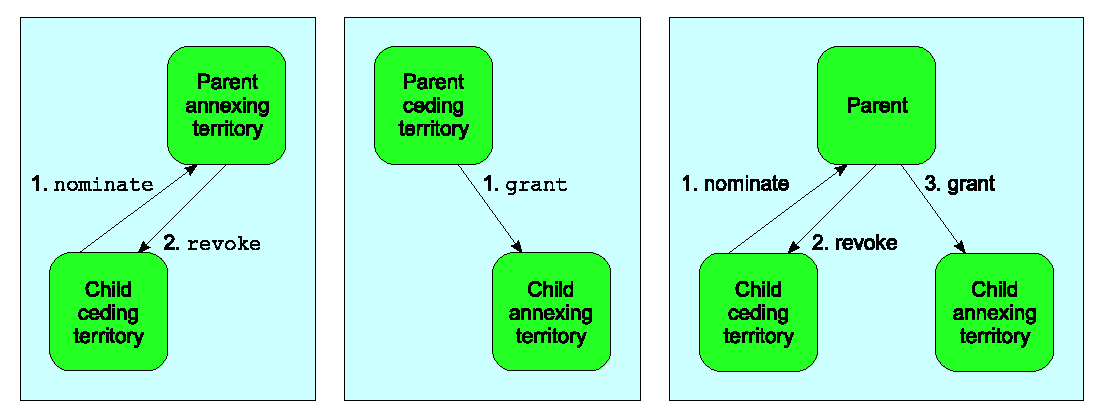
\includegraphics[width=\figwidth]{figures/grant-topdown}
\caption[Types of territory migrations]{Territory migrations are always driven by the parent in the namespace tree, which can annex a neighboring territory, cede territory to another envoy, or coordinates the transfer of a territory from one neighbor to another. For a child to initiate a transfer, it must send a \texttt{nominate} request to the parent, which then carries out the transfer.}
\label{fig:grant-topdown}
\end{figure}

\subsubsection{Transferring state}\label{sec:migrating-state}

When an envoy is granted a new territory, the first thing that it needs is a description of the boundaries. A territory is just a branch of the global namespace hierarchy, so it uniquelyuniquly identified by its root pathname. In addition to that, the parent envoy sends a list of exits from the territory. An exit is a link to an already-established territory that branches off from the one being granted. Since the boundary description may include any number of exits, multiple messages may be required to transmit the full set.

The new owner also receives a full set of active file handles for the new territory. With the 9p protocol, a file handle may identify a opened or unopened files, file or directories used for \texttt{walk} or \texttt{stat} calls, or directories in the process of being read. To facilitate territory changes and transparent crash recovery, the envoy must be able to recreate any state needed to continue a directory read from the number of bytes returned so far in the sequence of reads. Transfers are relatively rare, and transfers that interrupt \texttt{readdir} sequences are even less common, so the prototype simply starts from the beginning and throws away enough data to find the appropriate place in the directory when the need arises.

Every element of state transferred to the new owner, including the boundaries and the file handles, has a counterpart maintained by a partner envoy that must be notified of the changes. The root name comes from the parent, which already knows about the transfer (since it initiated it), but the boundary exits and file handles require that notifications be sent to their respective envoys. The previous owner is a special case, and since it is also identified in the grant sequence, the new owner can safely assume that the old has completely adjusted to the new order of things and not explicitly notify it of each file handle and shared border the two have in common. Some may also be local to the new owner; good territory assignments regularly bring the territory to the main user, so this is a good result for file handles. For all others, the grant recipient sends a notification immediately, grouping multiple entries going to the same remote envoy when appropriate.

The other side of the process is having a territory ownership revoked. As with all such operations, the process is coordinated by the parent. Viewed strictly as a bilateral arrangement, every revoke appears to the child as a merger of a subtree into its parent, though for convenience it is given a hint about where the territory is going to end up.

A revoke operation works much like a grant operation in reverse: the envoy receives a revoke message identifying the root of the territory, and it responds by sending back the current borders and active file handles. It updates its own state for local file handles that become remote, but otherwise leaves updates to the new owner as described above. This is important for synchronizing the transfer with client requests, as detailed below.

Together with \texttt{nominate} messages, grant and revoke transactions give full flexibility for arranging territories. An envoy may cede part of its territory by granting it to a remote envoy and establishing a parent/child relationship with it. An owner may likewise cede its territory to the parent or to a third envoy by issuing a nominate request. Compound requests that carve up territories in more detail are not directly supported, though some could be simulated through sequences of transactions. In general, complicated control decisions made by a central player are avoided in preference to localized choices. The owner of a territory is the only envoy that knows the recent history of requests, and is thus best suited to make realignment decisions.

\subsubsection{Inflight operations}

Top-down coordination of synchronized transactions helps prevent deadlock, but other synchronization issues still exist in territory boundary changes. File operations may be at any stage of completion when the transfer begins, and all must complete successfully without interrupting the client.

The prototype is designed to favor simplicity over other virtues in complex transactions, and this is no exception. Each participant in a migration waits for all inflight transactions directly involving the territory in question to complete before locking it and queuing up any further incoming requests. When the transfer is complete, the lock is released and the queue examined. Significantly, a revoke transaction always completes after a grant (when the two are paired) and after all other envoys involved have been notified of the change. For some requests this will result in nothing more than a pause, while for others the immediate consequence is a failed result. The envoy may no longer recognize a file handle that has been transferred, and can do no more than send the request back to its originator to try again. Note that forwarding it as a special case is an option, but a dangerous one. The message could still end up at the wrong place due to bad timing (and a second transfer of the target), it would involve just as many network round trips (originator to old owner to new owner vs.\ originator to old owner followed by originator to new owner), and the new owner would reject the request anyway as coming from the wrong owner (recall that remote file handles are associated with the client's envoy).

\figref{fig:migrate-sync} illustrates a request that conflicts with a territory transfer. A request coming from a client's envoy that reaches its target before the territory is locked is allowed to run to completion. If it arrives after the lock, then it is suspended (this is true if the territory owner is the same as the client's envoy, or if it is remote). The revoke transaction only completes after the corresponding grant has completed and the client's envoy has been notified of the update, so when the old owner bounces the request back, the client's envoy knows the new forwarding address and can immediately retry the request with the new owner. If a request comes after a particular file handle has been updated but before the grant has completed, the new owner simply holds the request until the transfer transaction is complete, at which point it can safely start processing requests, even before the revoke operation has been finalized.

\begin{figure}[tp]
\centering
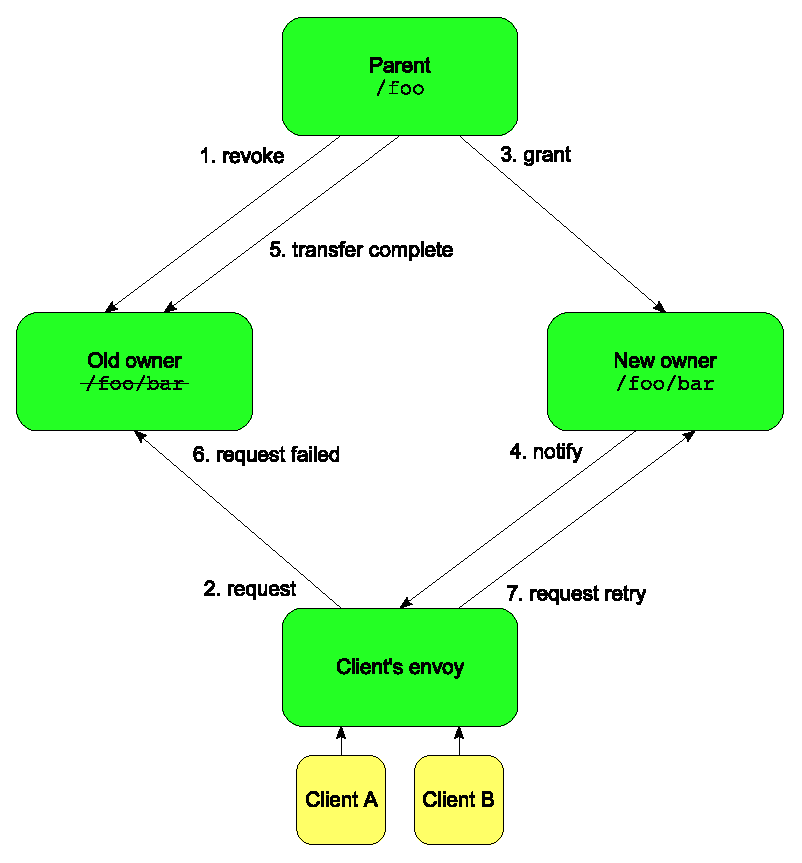
\includegraphics[width=\figwidth]{figures/migrate-sync}
\caption[Sequence of events in a territory migration]{The sequence of events when a client file request conflicts with a territory transfer.}
\label{fig:migrate-sync}
\end{figure}

\subsection{Limitations}

The prototype include some limitations that are artifacts of the implementation, rather than being inherent to the Envoy model. These are problems that can be solved with some routine engineering, and would need to be addressed in a production system. For the prototype, however, solving them would have added little value at the expense of extra complexity.

\subsubsection{Envoys as failure points}

The first issue is that a failing envoy loses all state for its local clients. This makes the failure of a single service affect all services on the same physical machine without an option for recovery. While services also depend on other node-wide management software, including the virtual machine manager, this is a dependency that could be removed.

The 9p protocol does not include any provision for recovering from a server failure, and the TCP connection used between the client and the envoy cannot be recovered transparently using standard network stacks. Both issues can be resolved by introducing a proxy between the client and the envoy (much as the envoy serves as a proxy for connections to remote envoys) that tracks the state of file handles, and is capable of restoring that state to a restarted envoy. Better yet, the client driver could be modified to maintain this state, and a recovery protocol introduced to synchronize and validate the state with a restarted envoy.

\subsubsection{Migrating clients}

A related problem is restoring state for VM instances that have been migrated to a different machine. With the current prototype, those instances will continue to send all requests to the envoy on the old machine, as they will not be aware of the migration. The envoys could easily transfer the state by employing a mechanism similar to that used to transfer territories, but a way to detect the migration would be necessary, probably through direct cooperation with the management process invoking the migration. The IP address of the new envoy would be different than the old, so some cooperation from the client would also be necessary to restart the TCP connection. Tricks involving the virtual network device connecting the client to the envoy may also be possible, but it is unlikely that the additional transparency gained would be worth the complexity introduced.

A related problem is virtual machines that are suspended to disk and restarted later, on either the same or a different physical machine. This can be viewed as another form of client migration, but from the client's perspective it more closely resembles the condition when the envoy fails and restarts. The solution proposed for that---clients retaining copies of file handle state and envoys validating and accepting it---would also be applicable here.

\subsubsection{Control of administrative directories}

For simplicity, territories control is only transferred starting at an image root, so all administrative directories are controlled by a single envoy. Traffic to these levels of the hierarchy are normally confined to mount requests and administrative actions, and for the latter most of the work for snapshot creation and removal is still done by territory owners.

Still, nothing precludes this area from being split up. Tracking authentication credentials and resolving the target of fork requests would become a bit more complex, but not substantially so.

The more serious issue is that the prototype cannot migrate control of the root to another envoy. The standard mechanism for migrating territories is applicable, but in addition all envoys would need to be notified of the change so that mount requests (which always start from the root of the namespace) could be properly routed. Straightforward solutions exist, but they were of little value in accomplishing the goals of the prototype and so were not pursued.

\section{Summary}